\documentclass[tikz,border=0pt]{standalone}
\usepackage{xcolor}
\usetikzlibrary{calc}
% Palette: Sam_Comm_final.png by eye, and the drones and raiders.
\definecolor{ink}{HTML}{3B2340}
\definecolor{sky}{HTML}{EFC46A}
\definecolor{skyhi}{HTML}{F5DA92}
\definecolor{skylow}{HTML}{E9B060}
\definecolor{cloud}{HTML}{F2D58A}
\definecolor{paper}{HTML}{FBEFD0}
\definecolor{cream}{HTML}{FFF6E0}
\definecolor{white}{HTML}{FFFFFF}
\definecolor{wallA}{HTML}{E88A73}
\definecolor{wallB}{HTML}{EE9F7E}
\definecolor{wallC}{HTML}{E47A7E}
\definecolor{wallD}{HTML}{F0B07E}
\definecolor{wallE}{HTML}{D9765F}
\definecolor{wallF}{HTML}{E99A8A}
\definecolor{greenA}{HTML}{8DBB7E}
\definecolor{greenB}{HTML}{6FA77A}
\definecolor{greenC}{HTML}{A9C97F}
\definecolor{greenD}{HTML}{5E9C6A}
\definecolor{greenE}{HTML}{4A8060}
\definecolor{sage}{HTML}{9DB98A}
\definecolor{sagedark}{HTML}{6F8F66}
\definecolor{sagelight}{HTML}{C2D6A6}
\definecolor{window}{HTML}{F6E7A0}
\definecolor{windark}{HTML}{8C5A64}
\definecolor{metal}{HTML}{8D9A93}
\definecolor{metaldark}{HTML}{5E6B66}
\definecolor{metallight}{HTML}{B9C4BC}
\definecolor{wood}{HTML}{B9835A}
\definecolor{wooddark}{HTML}{8C5A3C}
\definecolor{woodlight}{HTML}{D9A66F}
\definecolor{stone}{HTML}{E7C9A0}
\definecolor{stonedark}{HTML}{C9A47E}
\definecolor{concrete}{HTML}{D8C3A4}
\definecolor{concretedark}{HTML}{B8A084}
\definecolor{asphalt}{HTML}{8E7A86}
\definecolor{asphaltdark}{HTML}{6E5C68}
\definecolor{roadline}{HTML}{F6E7A0}
\definecolor{kerb}{HTML}{D8B48C}
\definecolor{red}{HTML}{E0483E}
\definecolor{redlight}{HTML}{F27A6A}
\definecolor{gold}{HTML}{FFB000}
\definecolor{goldlight}{HTML}{FFD54F}
\definecolor{teal}{HTML}{4FA3A0}
\definecolor{tealdark}{HTML}{3C8582}
\definecolor{magenta}{HTML}{FF2E88}
\definecolor{cyan}{HTML}{13CFE3}
\definecolor{violet}{HTML}{8A5BD6}
\definecolor{orange}{HTML}{F2803A}
\definecolor{pink}{HTML}{F48FB1}
\definecolor{glow}{HTML}{4FE6E0}
\definecolor{glowhi}{HTML}{C8FFF9}
\definecolor{hot}{HTML}{FF6A1A}
\definecolor{hothi}{HTML}{FFD07A}
\definecolor{armour}{HTML}{7E7A86}
\definecolor{armourdark}{HTML}{5A5466}
\definecolor{armourlight}{HTML}{A8A2B0}
\definecolor{wasp}{HTML}{E0A82E}
\definecolor{waspdark}{HTML}{B07E1A}
\definecolor{moth}{HTML}{F2E6C8}
\definecolor{mothdark}{HTML}{D2C09A}
\definecolor{hornet}{HTML}{3C8582}
\definecolor{hornetdark}{HTML}{2C6260}
\definecolor{warden}{HTML}{E47A7E}
\definecolor{wardendark}{HTML}{B85A62}
\definecolor{tick}{HTML}{8DBB7E}
\definecolor{tickdark}{HTML}{5E8A5A}
\definecolor{strider}{HTML}{D9765F}
\definecolor{striderdark}{HTML}{A8543F}
\definecolor{queen}{HTML}{7E5C94}
\definecolor{queendark}{HTML}{4C3A60}
\definecolor{jacket}{HTML}{6FA77A}
\definecolor{jacketb}{HTML}{4FA3A0}
\definecolor{jacketc}{HTML}{E88A73}
\definecolor{jacketd}{HTML}{F0B07E}
\definecolor{skin}{HTML}{F2C49A}
\definecolor{skinb}{HTML}{C98C6A}
\definecolor{skinc}{HTML}{8C5A3C}
\definecolor{hair}{HTML}{3B2340}
\definecolor{goo}{HTML}{B6E35A}
\definecolor{goodark}{HTML}{7FB23A}
\newcommand{\Ink}{1.6pt}
\tikzset{inked/.style={draw=ink, line width=\Ink, line join=round, line cap=round}}
\begin{document}
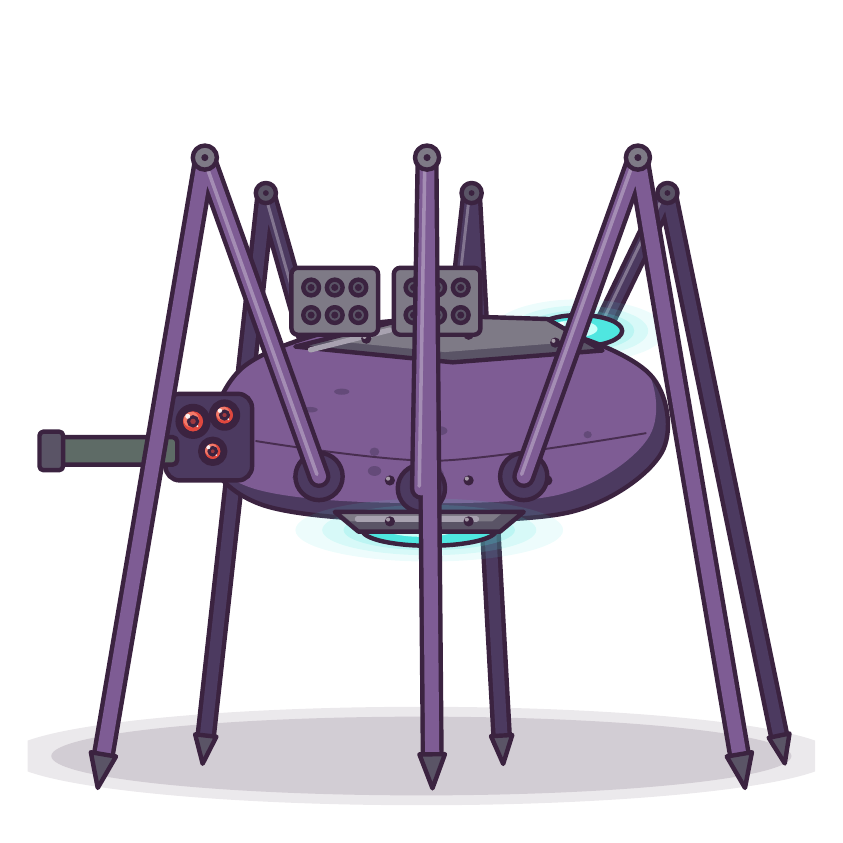
\begin{tikzpicture}
\clip (0,0) rectangle (10,10);
\begin{scope}[shift={(0,0)}, scale=1]
\fill[ink, opacity=0.10] (5,0.75) ellipse (5.264 and 0.625);
\fill[ink, opacity=0.14] (5,0.75) ellipse (4.7 and 0.5);
\draw[ink, line width=7.468pt, line cap=round, line join=round] (3.95,4.65) -- (3.025,7.9) -- (2.255,0.95);
\draw[queendark, line width=4.268pt, line cap=round, line join=round] (3.95,4.65) -- (3.025,7.9) -- (2.255,0.95);
\draw[white, opacity=0.3, line width=1.067pt, line cap=round] (3.928,4.672) -- (3.003,7.923);
\filldraw[inked,fill=armourdark] (3.025,7.9) circle (0.128);
\fill[ink] (3.025,7.9) circle (0.037);
\filldraw[inked,fill=armourdark] (2.396,0.995) -- (2.222,0.652) -- (2.127,1.025) -- cycle;
\draw[ink, line width=7.468pt, line cap=round, line join=round] (5.25,4.5) -- (5.638,7.9) -- (6.022,0.95);
\draw[queendark, line width=4.268pt, line cap=round, line join=round] (5.25,4.5) -- (5.638,7.9) -- (6.022,0.95);
\draw[white, opacity=0.3, line width=1.067pt, line cap=round] (5.228,4.522) -- (5.615,7.923);
\filldraw[inked,fill=armourdark] (5.638,7.9) circle (0.128);
\fill[ink] (5.638,7.9) circle (0.037);
\filldraw[inked,fill=armourdark] (6.154,1.017) -- (6.039,0.65) -- (5.884,1.002) -- cycle;
\draw[ink, line width=7.468pt, line cap=round, line join=round] (6.55,4.65) -- (8.125,7.9) -- (9.555,0.95);
\draw[queendark, line width=4.268pt, line cap=round, line join=round] (6.55,4.65) -- (8.125,7.9) -- (9.555,0.95);
\draw[white, opacity=0.3, line width=1.067pt, line cap=round] (6.527,4.672) -- (8.102,7.923);
\filldraw[inked,fill=armourdark] (8.125,7.9) circle (0.128);
\fill[ink] (8.125,7.9) circle (0.037);
\filldraw[inked,fill=armourdark] (9.675,1.036) -- (9.615,0.656) -- (9.411,0.982) -- cycle;
\fill[glow, opacity=0.1] (7,6.15) ellipse (1.1 and 0.4);
\fill[glow, opacity=0.14] (7,6.15) ellipse (0.88 and 0.32);
\fill[glow, opacity=0.2] (7,6.15) ellipse (0.704 and 0.256);
\filldraw[inked,fill=glow] (7,6.15) ellipse (0.55 and 0.2);
\fill[glowhi]  (6.934,6.174) ellipse (0.303 and 0.11);
\fill[white, opacity=0.9] (6.78,6.23) circle (0.036);
\fill[queendark] plot[smooth cycle, tension=0.55] coordinates {(2.3,4.6) (2.75,5.7) (4.4,6.25) (6.5,6.2) (7.9,5.6) (8.05,4.6) (6.9,3.85) (4.6,3.75) (2.95,3.95)};
\begin{scope}\clip plot[smooth cycle, tension=0.55] coordinates {(2.3,4.6) (2.75,5.7) (4.4,6.25) (6.5,6.2) (7.9,5.6) (8.05,4.6) (6.9,3.85) (4.6,3.75) (2.95,3.95)};
\begin{scope}[shift={(-0.15,0.22)}]\fill[queen] plot[smooth cycle, tension=0.55] coordinates {(2.3,4.6) (2.75,5.7) (4.4,6.25) (6.5,6.2) (7.9,5.6) (8.05,4.6) (6.9,3.85) (4.6,3.75) (2.95,3.95)};\end{scope}
\end{scope}
\draw[inked] plot[smooth cycle, tension=0.55] coordinates {(2.3,4.6) (2.75,5.7) (4.4,6.25) (6.5,6.2) (7.9,5.6) (8.05,4.6) (6.9,3.85) (4.6,3.75) (2.95,3.95)};
\begin{scope}\clip plot[smooth cycle, tension=0.55] coordinates {(2.3,4.6) (2.75,5.7) (4.4,6.25) (6.5,6.2) (7.9,5.6) (8.05,4.6) (6.9,3.85) (4.6,3.75) (2.95,3.95)};
\begin{scope}\clip plot[smooth cycle, tension=0.55] coordinates {(2.3,4.6) (2.75,5.7) (4.4,6.25) (6.5,6.2) (7.9,5.6) (8.05,4.6) (6.9,3.85) (4.6,3.75) (2.95,3.95)};
\fill[queendark, opacity=0.5] (7.112,4.831) ellipse (0.052 and 0.046);
\fill[queendark, opacity=0.5] (4.405,4.37) ellipse (0.085 and 0.063);
\fill[queendark, opacity=0.5] (3.587,5.148) ellipse (0.097 and 0.035);
\fill[queendark, opacity=0.5] (3.434,4.284) ellipse (0.074 and 0.037);
\fill[queendark, opacity=0.5] (3.989,5.377) ellipse (0.097 and 0.039);
\fill[queendark, opacity=0.5] (5.028,5.825) ellipse (0.074 and 0.043);
\fill[queendark, opacity=0.5] (3.641,4.672) ellipse (0.075 and 0.046);
\fill[queendark, opacity=0.5] (4.404,4.614) ellipse (0.062 and 0.054);
\fill[queendark, opacity=0.5] (5.224,4.881) ellipse (0.107 and 0.059);
\fill[queendark, opacity=0.5] (5.191,4.334) ellipse (0.093 and 0.066);
\end{scope}
\fill[white, opacity=0.28] (5.1,6.05) ellipse (1.1 and 0.12);
\end{scope}
\fill[armourdark] (3.4,5.95) -- (5,6.35) -- (6.6,6.3) -- (7.3,5.9) -- (5.4,5.75) -- cycle;
\begin{scope}\clip (3.4,5.95) -- (5,6.35) -- (6.6,6.3) -- (7.3,5.9) -- (5.4,5.75) -- cycle;
\begin{scope}[shift={(-0.1,0.13)}]\fill[armour] (3.4,5.95) -- (5,6.35) -- (6.6,6.3) -- (7.3,5.9) -- (5.4,5.75) -- cycle;\end{scope}
\end{scope}
\draw[inked] (3.4,5.95) -- (5,6.35) -- (6.6,6.3) -- (7.3,5.9) -- (5.4,5.75) -- cycle;
\draw[armourlight, line width=1.92pt, line cap=round] (3.592,5.908) -- (4.6,6.16);
\fill[ink] (4.3,6.05) circle (0.065);
\fill[white, opacity=0.55] (4.277,6.073) circle (0.026);
\fill[ink] (5.6,6.1) circle (0.065);
\fill[white, opacity=0.55] (5.577,6.123) circle (0.026);
\fill[ink] (6.7,6) circle (0.065);
\fill[white, opacity=0.55] (6.677,6.023) circle (0.026);
\draw[ink, line width=0.7pt, line cap=round, line join=round, opacity=0.8] plot[smooth, tension=0.5] coordinates {(2.9,4.75) (5.2,4.5) (7.85,4.85)};
\fill[ink] (3.6,4.25) circle (0.065);
\fill[white, opacity=0.55] (3.577,4.273) circle (0.026);
\fill[ink] (4.6,4.25) circle (0.065);
\fill[white, opacity=0.55] (4.577,4.273) circle (0.026);
\fill[ink] (5.6,4.25) circle (0.065);
\fill[white, opacity=0.55] (5.577,4.273) circle (0.026);
\fill[ink] (6.6,4.25) circle (0.065);
\fill[white, opacity=0.55] (6.577,4.273) circle (0.026);
\fill[glow, opacity=0.1] (5.1,3.62) ellipse (1.7 and 0.4);
\fill[glow, opacity=0.14] (5.1,3.62) ellipse (1.36 and 0.32);
\fill[glow, opacity=0.2] (5.1,3.62) ellipse (1.088 and 0.256);
\filldraw[inked,fill=glow] (5.1,3.62) ellipse (0.85 and 0.2);
\fill[glowhi]  (4.998,3.644) ellipse (0.468 and 0.11);
\fill[white, opacity=0.9] (4.76,3.7) circle (0.036);
\fill[armourdark] (3.9,3.85) -- (6.3,3.85) -- (6,3.6) -- (4.2,3.6) -- cycle;
\begin{scope}\clip (3.9,3.85) -- (6.3,3.85) -- (6,3.6) -- (4.2,3.6) -- cycle;
\begin{scope}[shift={(-0.1,0.13)}]\fill[armour] (3.9,3.85) -- (6.3,3.85) -- (6,3.6) -- (4.2,3.6) -- cycle;\end{scope}
\end{scope}
\draw[inked] (3.9,3.85) -- (6.3,3.85) -- (6,3.6) -- (4.2,3.6) -- cycle;
\draw[armourlight, line width=1.92pt, line cap=round] (4.188,3.76) -- (5.7,3.76);
\fill[ink] (4.6,3.73) circle (0.065);
\fill[white, opacity=0.55] (4.577,3.753) circle (0.026);
\fill[ink] (5.6,3.73) circle (0.065);
\fill[white, opacity=0.55] (5.577,3.753) circle (0.026);
\filldraw[inked,fill=armour,rounded corners=0.08cm] (3.35,6.1) rectangle (4.45,6.95);
\filldraw[inked,fill=armourdark] (3.6,6.35) circle (0.1);
\fill[ink] (3.6,6.35) circle (0.045);
\filldraw[inked,fill=armourdark] (3.9,6.35) circle (0.1);
\fill[ink] (3.9,6.35) circle (0.045);
\filldraw[inked,fill=armourdark] (4.2,6.35) circle (0.1);
\fill[ink] (4.2,6.35) circle (0.045);
\filldraw[inked,fill=armourdark] (3.6,6.7) circle (0.1);
\fill[ink] (3.6,6.7) circle (0.045);
\filldraw[inked,fill=armourdark] (3.9,6.7) circle (0.1);
\fill[ink] (3.9,6.7) circle (0.045);
\filldraw[inked,fill=armourdark] (4.2,6.7) circle (0.1);
\fill[ink] (4.2,6.7) circle (0.045);
\filldraw[inked,fill=armour,rounded corners=0.08cm] (4.65,6.1) rectangle (5.75,6.95);
\filldraw[inked,fill=armourdark] (4.9,6.35) circle (0.1);
\fill[ink] (4.9,6.35) circle (0.045);
\filldraw[inked,fill=armourdark] (5.2,6.35) circle (0.1);
\fill[ink] (5.2,6.35) circle (0.045);
\filldraw[inked,fill=armourdark] (5.5,6.35) circle (0.1);
\fill[ink] (5.5,6.35) circle (0.045);
\filldraw[inked,fill=armourdark] (4.9,6.7) circle (0.1);
\fill[ink] (4.9,6.7) circle (0.045);
\filldraw[inked,fill=armourdark] (5.2,6.7) circle (0.1);
\fill[ink] (5.2,6.7) circle (0.045);
\filldraw[inked,fill=armourdark] (5.5,6.7) circle (0.1);
\fill[ink] (5.5,6.7) circle (0.045);
\filldraw[inked,fill=queendark,rounded corners=0.18cm] (1.75,4.25) rectangle (2.85,5.35);
\filldraw[inked,fill=metaldark,rounded corners=0.06cm] (0.35,4.45) rectangle (1.9,4.8);
\filldraw[inked,fill=armourdark,rounded corners=0.05cm] (0.15,4.38) rectangle (0.45,4.87);
\filldraw[inked,fill=armourdark] (2.1,5) circle (0.195);
\filldraw[inked,fill=red] (2.1,5) circle (0.16);
\fill[redlight] (2.076,5.024) circle (0.099);
\fill[red!60!ink] (2.108,4.992) circle (0.058);
\draw[ink, line width=1.12pt] (2.1,5) circle (0.058);
\fill[white, opacity=0.9] (2.033,5.064) circle (0.032);
\fill[white, opacity=0.9] (2.156,4.939) circle (0.014);
\draw[inked] (2.1,5) circle (0.16);
\filldraw[inked,fill=armourdark] (2.5,5.08) circle (0.171);
\filldraw[inked,fill=red] (2.5,5.08) circle (0.14);
\fill[redlight] (2.479,5.101) circle (0.087);
\fill[red!60!ink] (2.507,5.073) circle (0.05);
\draw[ink, line width=1.12pt] (2.5,5.08) circle (0.05);
\fill[white, opacity=0.9] (2.441,5.136) circle (0.028);
\fill[white, opacity=0.9] (2.549,5.027) circle (0.013);
\draw[inked] (2.5,5.08) circle (0.14);
\filldraw[inked,fill=armourdark] (2.35,4.62) circle (0.159);
\filldraw[inked,fill=red] (2.35,4.62) circle (0.13);
\fill[redlight] (2.331,4.639) circle (0.081);
\fill[red!60!ink] (2.357,4.614) circle (0.047);
\draw[ink, line width=1.12pt] (2.35,4.62) circle (0.047);
\fill[white, opacity=0.9] (2.295,4.672) circle (0.026);
\fill[white, opacity=0.9] (2.396,4.571) circle (0.012);
\draw[inked] (2.35,4.62) circle (0.13);
\filldraw[inked,fill=queendark] (3.7,4.3) circle (0.3);
\fill[ink] (3.7,4.3) circle (0.08);
\fill[white, opacity=0.55] (3.672,4.328) circle (0.032);
\draw[ink, line width=8.322pt, line cap=round, line join=round] (3.7,4.3) -- (2.25,8.35) -- (0.95,0.7);
\draw[queen, line width=5.122pt, line cap=round, line join=round] (3.7,4.3) -- (2.25,8.35) -- (0.95,0.7);
\draw[white, opacity=0.3, line width=1.28pt, line cap=round] (3.673,4.327) -- (2.223,8.377);
\filldraw[inked,fill=armour] (2.25,8.35) circle (0.153);
\fill[ink] (2.25,8.35) circle (0.045);
\filldraw[inked,fill=armourdark] (1.122,0.744) -- (0.89,0.345) -- (0.802,0.798) -- cycle;
\filldraw[inked,fill=queendark] (5,4.15) circle (0.3);
\fill[ink] (5,4.15) circle (0.08);
\fill[white, opacity=0.55] (4.972,4.178) circle (0.032);
\draw[ink, line width=8.322pt, line cap=round, line join=round] (5,4.15) -- (5.072,8.35) -- (5.138,0.7);
\draw[queen, line width=5.122pt, line cap=round, line join=round] (5,4.15) -- (5.072,8.35) -- (5.138,0.7);
\draw[white, opacity=0.3, line width=1.28pt, line cap=round] (4.973,4.177) -- (5.045,8.377);
\filldraw[inked,fill=armour] (5.072,8.35) circle (0.153);
\fill[ink] (5.072,8.35) circle (0.045);
\filldraw[inked,fill=armourdark] (5.299,0.773) -- (5.141,0.34) -- (4.975,0.771) -- cycle;
\filldraw[inked,fill=queendark] (6.3,4.3) circle (0.3);
\fill[ink] (6.3,4.3) circle (0.08);
\fill[white, opacity=0.55] (6.272,4.328) circle (0.032);
\draw[ink, line width=8.322pt, line cap=round, line join=round] (6.3,4.3) -- (7.75,8.35) -- (9.05,0.7);
\draw[queen, line width=5.122pt, line cap=round, line join=round] (6.3,4.3) -- (7.75,8.35) -- (9.05,0.7);
\draw[white, opacity=0.3, line width=1.28pt, line cap=round] (6.273,4.327) -- (7.723,8.377);
\filldraw[inked,fill=armour] (7.75,8.35) circle (0.153);
\fill[ink] (7.75,8.35) circle (0.045);
\filldraw[inked,fill=armourdark] (9.198,0.798) -- (9.11,0.345) -- (8.878,0.744) -- cycle;
\end{scope}
\end{tikzpicture}
\end{document}
